%\documentclass[options]{class}
\documentclass[10pt,letterpaper,twocolumn]{article}

%Paquete de Idioma
\usepackage[english, en-table]{babel}

%Codificación Alfabeto
\usepackage[utf8]{inputenc}

%Codificación de Fuente
\usepackage[T1]{fontenc}

%Índice
\usepackage{makeidx}

%Gráficos
\usepackage{graphicx}
\usepackage{float} 
%\usepackage{xcolor} 
\usepackage{multirow} 
\usepackage{multicol} 
\usepackage[table]{xcolor}
\usepackage[pdftex]{hyperref}
\usepackage{color}
\usepackage{colortbl}
\usepackage{authblk}
\usepackage{pgfplots}
\usepackage{mathtools}
\usepackage{graphicx}
\usepackage{subfigure}
\usepackage{hyperref}
\usepackage{enumerate}
\usepackage{vmargin}

%Matemática
\usepackage{geometry,pdfpages}
\usepackage{amsmath}
\usepackage{amsfonts}
\usepackage{amssymb}
%\usepackage{amstext} 

%Estilo de Página Numeración superior

\renewcommand{\thesection}{\Roman{section}}

\setpapersize{A4}
\setmargins{1.5 cm}       
{1.0 cm}                       
{18 cm}                      
{25.5 cm}
{5pt}
{0.5 cm}                           
{100 pt}                             
{0cm}                          

%Hiperlinks \href{url}{text}
\usepackage[pdftex]{hyperref}
\pgfplotsset{compat=1.16} 

\begin{document}
%Titulo
\title{\textbf{\large{Hints on halo evolution in SFDM models with galaxy observations}}}
%Autor
\author[1]{\small {Alma X. Gónzalez-Morales}}
\author[2]{Alberto Diez-Tejedor}
\author[3]{L. Arturo Ureña-López}
\author[4]{Octavio Valenzuela}
\affil[1]{\footnotesize {Instituto de Ciencias Nucleares Universidad Nacional Autónoma de México, Circuito Exterior C.U., A.P. 70-543, México D.F. 04510, México}}
\affil[2-3]{Departamento de Física, División de Ciencias e Ingenierías, Campus León, Universidad de Guanajuato, León 37150, México}
\affil[4]{Instituto de Astronomía, Universidad Nacional Autónoma de México, Circuito Exterior C.U., A.P. 70-264,México D.F. 04510, México \vspace{-2em}}
\date{\small{(Dated: October 29, 2018)}}\vspace{-3em}

\twocolumn[
  \begin{@twocolumnfalse}
    \maketitle 
    \renewcommand{\abstractname}{}
    \begin{abstract}
A massive, self-interacting scalar field has been considered as a possible candidate for the dark
matter in the universe. We present an observational constraint to the model arising from strong
lensing observations in galaxies. The result points to a discrepancy in the properties of scalar field dark matter halos for dwarf and lens galaxies, mainly because halo parameters are directly related to physical quantities in the model. This is an important indication that it becomes necessary to have a better understanding of halo evolution in scalar field dark matter models, where the presence of baryons can play an important role.
\\PACS numbers: 95.30.Sf, 95.35.+d, 98.62.Gq, 98.62.Sb.
    \end{abstract}
  \end{@twocolumnfalse}
  ]\\
\section[I]{\centering \small {INTRODUCTION}}
The nature of dark matter (DM) remains elusive today,
even though a generic cold particle weakly coupled to the
standard model seems to be the most promising candidate
\cite{1}. Treating DM as a bunch of classical particles is
an appropriate effective description for many physical situations.
However, if DM is composed of bosons, the zero
mode can develop a non-vanishing expectation value; this
effect is usually known as Bose-Einstein condensation. A
condensed phase does not admit a description in terms
of classical particles, and the concept of a coherent excitation
(i.e. a classical field) is more appropriate for practical
purposes \cite{2}. A specific realization of this scenario
can be provided by the axion \cite{3}, see also \cite{4}.
In this paper we shall explore the lensing properties
of a generic model of DM particles in a condensate, and
compare the conditions necessary to produce strong lensing
with those required to explain the dynamics of dwarf
galaxies. As a result we will get some insight into halo
evolution arising from this type of models.
In particular, we will consider the case of a complex,
massive, self-interacting scalar field $\phi$ satisfying
the Klein-Gordon (KG) equation, $\square\phi - (mc/\hbar)^{2}\phi - \lambda|\phi^{2}\phi = 0$, with the box denoting the d'Alembertian
operator in four dimensions. For those natural situations
in which the scalar field mass $m$ is much smaller
than the Planck scale, $m_{Planck} = (\hbar c/G)^{1/2}$, such that
$\Lambda\equiv\lambda{m^2_{Planck}/4\pi{m^2}}\gg1$, the coherent (self-gravitating, spherically symmetric) solutions to the KG equation admit a very simple expression for the mass density [5, 6],

\begin{eqnarray}
\label{eq:1}
\rho(r)=\left\lbrace\begin{array}{rl}
\rho_{c}\frac{sin(\pi{r}/r_{max})}{(\pi{r}/r_{max})}~for~ r<r_{max}\\0~~~~~~~~~for~r\geq{r_{max}}\end{array}\right.
\end{eqnarray}
\\
As usual we will refer to this model as scalar field dark matter (SFDM). Here $r_{max}\equiv\sqrt{\pi^2\Lambda/2}(\hbar/mc)$ is a constant with dimensions of length (notice that $r_{max}$ is just the Compton wavelength of the scalar particle, $\hbar/mc$, scaled by a factor of order $\Lambda^1/2$, and $\rho_{c}$ the density at the center of the configuration. The mass density profile in Eq. (\ref{eq:1}) leads to compact objects of size $r_{max}$, and typical masses, $4\rho_{c}r^3_{max}/\pi$, that vary from configuration to configuration according to the value of the central density. 

Eq. (\ref{eq:1}) was obtained without taking into account the gravitational in influence of any other matter sources, and assuming that all the scalar particles are in the condensate. It has been used as a first order approximation to describe the distribution of matter in dwarf shperoidals, which are expected to be DM dominated [6-8]. The mass distribution would be smooth close to the center of these galaxies, alleviating the cusp/core problem motivated by the discrepancies between the observed high resolution rotation curves and the profiles suggested by N-body simulations
\cite{9}; see however \cite{10}.\\\\
The dynamics of dwarf galaxies suggests a self interacting
scalar with $m^{4}/\lambda ~ 50 - 75 (eV/c^{2})^{4}$, (i.e. $r_{max} ~ 5.5 - 7Kpc$  and typical central densities of the
order of $\rho_{c} ~ 10^{-13} M_{\odot}/pc^3$ see Ref. \cite{6}. We are aware
that Milky Way size galaxies are, at least, an order of
magnitude larger than this value of $r_{max}$, and then they do not fit in this model as it stands. Nonetheless, if not all the DM particles are in the condensate, there is a possibility to have gravitational configurations where the inner regions are still described by the mass density profile in Eq. (\ref{eq:1}), wrapped in a cloud of non-condensed particles \cite{11}. For the purpose of this paper we do not
need to specify the complete halo model. This is because
strong lensing is not very sensitive to the mass distribution
outside the Einstein radius, at most of the order of
a few Kpc, just bellow the expected value of $r_{max}$. We
could not neglect the exterior profile of the halo if we were
interested, for instance, in weak lensing observations.
\section[II]{\centering \small {LENSING PROPERTIES OF SFDM HALOS}}
In the weak field limit the gravitational lensing produced
by a mass distribution can be read directly from
the density profile. As usual we assume spherical symmetry,
and use the thin lens approximation, that is, the size
of the object is negligible when compared to the other
length scales in the configuration, i.e. the (angular) distances
between the observer and the lens, $D_{OL}$, the lens
and the source, $D_{LS}$, and from the observer to the source,
$D_{OS}$.\\
Under these assumptions the lens equation takes the
form
\begin{eqnarray}
\label{eq:2}
\beta=\theta-\frac{M(\theta)}{\pi{D^{2}_{OL}}\theta\Sigma_{cr}},
\end{eqnarray}
with $\beta$ and $\theta$ denoting the actual (unobservable) angular position of the source, and the apparent (observable) angular position of the image, respectively, both measured with respect to the line-of-sight \cite{12}. The (projected) mass enclosed in a circle of radius $\xi$, $M(\xi)$, is defined from the (projected) surface mass density, $\Sigma(\xi)$, through

\begin{eqnarray}
\label{eq:3}
\Sigma(\xi)\equiv\int^{\infty}_{-\infty}dz~\rho(z,\xi),~~M(\xi)\equiv2\pi\int^{\xi}_{0}d\xi'\xi'\Sigma(\xi').
\end{eqnarray}

Here $\xi = D_{OL}\theta$ is a radial coordinate in the lens plane, and $z$ a coordinate in the orthogonal direction. Finally $\Sigma_{cr} \equiv c^{2}D_{OS}/4\pi{G}D_{OL}D_{LS}$ is a critical value for the surface density.\\
In general, Eq. (\ref{eq:2}) will be non-linear in $\theta$, and it could be possible that for a given position of the source, $\beta$, there
would be multiple solutions (i.e. multiple images) for
the angle $\theta$. This is what happens in the strong lensing regime to be discussed below. One particular case is that with a perfect alignment between the source and the lens, that actually defines the Einstein ring, with an angular radius of $\theta_{E}\equiv \theta (\beta = 0)$.\\
For a SFDM halo, and in terms of the normalized lengths $\xi_{*}\equiv\xi/r_{max}~and~z_{*}\equiv z/r_{max}$, the surface mass density takes the form
\begin{eqnarray}
\label{eq:4}
\Sigma_{SDFM}(\xi_{*})=\frac{2\rho_{c}r_{max}}{\pi}\int^{z_{max}}_{0}\frac{sin(\pi\sqrt{\xi^{2}_{*}}+z^{2}_{*})}{\sqrt{\xi^{2}_{*}+z^{2}_{*}}}dz_{*},
\end{eqnarray}
with $0\leq\xi_{*}\leq1$ and $z_{max}=\sqrt{1-\xi^{2}_{*}}$. A similar expression can be obtained for the mass enclosed in a circle or radius $\xi$, see Eq. (3) above. Here we are not considering the effect of a scalar cloud surrounding the
condensate. For $r\lesssim{r_{max}}$ this will appear as a projection effect, which is usually considered to be small \cite{13}. Indeed, we have corroborated that the inclusion of an outer isothermal sphere does not affect the conclusions of this paper.\\ 
With the use of the expression for the projected mass, $M_{SFDM}(\xi_{*})$, the lens equation simplifies to
\begin{equation}
\tag{5a}\label{eq:5a}
\beta_{*}(\theta_{*})=\theta_{*}-\bar{\lambda}\frac{m(\theta_{*})}{\theta_{*}},
\end{equation}

\begin{figure}[h]
    \centering
    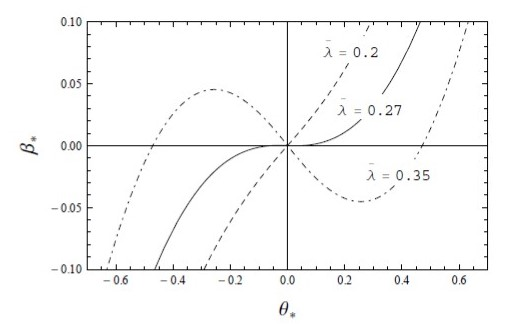
\includegraphics[width=0.4\textwidth]{Figura 1.jpg}
    \caption{The lens equation of a SFDM halo model, Eq. (5), as
a function of $\bar{\lambda}$. The roots define the Einstein radius, $\theta_{*E}$, and its local maximum (minimum) the critical impact parameter, $\beta_{*cr}$. Both quantities are well defined only for values of $\bar{\lambda}>\bar{\lambda}_{cr}\simeq0.27$, which is the threshold value for strong lensing.}
    \label{Fig. 1}
\end{figure}

where $m(\xi_{*})\equiv M_{SFDM}(\xi_{*})/\rho_{c}{r^{3}_{max}}$ is a normalized mass function, evaluated numerically. Here $ \beta_{*}= D_{OL}\beta/r_{max}$ and $\theta_{*}= D_{OL}\theta/r_{max}$ are the normalized angular positions of the source and images, respectively, and the parameter $\bar{\lambda}$ is given by

\begin{equation}
\tag{5b}\label{eq:5b}\small
\bar{\lambda}\equiv\frac{\rho_{c}r_{max}}{\pi\Sigma_{cr}}=0.57h^{-1}=\left\lgroup\frac{\rho_{c}}{M_{\odot}pc^{-3}}\right\rgroup\left\lgroup\frac{r_{max}}{kpc}\right\rgroup\frac{d_{OL}d_{LS}}{d_{OS}}.
\end{equation}

In order to avoid confusion with the self-interaction term, $\lambda$, we have introduced a bar in the new parameter $\bar{\lambda}$. We have also defined the reduced angular distances $d_{A}\equiv D_{A}H_{0}/c$, and considered $H_{0}\equiv100h(km/s)/Mpc$ as the Hubble constant today, with $h = 0.710\pm0.025$ \cite{14}.\\
In Fig. \ref{Fig. 1} we show the behavior of the lens equation (5) as the $\lambda$ parameter varies (i.e. for different values of the combination $\rho c r_{max})$. Some notes are in turn: $i$) Strong lensing can be produced only for configurations with $\bar{\lambda} > \bar{\lambda}_{cr} \simeq 0.27$, and $ii$) For these configurations, only those with an impact parameter $|\beta_{*}|<\beta_{*cr}$ can produce three images (note that the actual value of $\beta_{*cr}$ depends on the parameter $\bar{\lambda}, \beta_{*cr}(\bar{\lambda}))$.
These conditions on the SFDM profile are very similar to those obtained for the Burkert model in \cite{15}; this is not surprising because both of them have a core in radius. In that sense SFDM halos are analogous to those proposed by Burkert \cite{16}, but with the advantage that their properties are clearly connected to physical parameters in the model. 
In Fig. \ref{Fig. 2} we show the magnitude of the Einstein radius, $\theta_{*E}$, as a function of the parameter $\bar{\lambda}$, where for comparison we have also plotted the same quantity for the NFW \cite{17} and Burkert \cite{15} profiles. The minimum value of $\bar{\lambda}$ needed to produce multiple images is higher for a SFDM halo, $\bar{\lambda}^{NFW}_{cr} = 0 < \bar{\lambda}^{Burkert}_{cr} = 2/\pi^{2} < \bar{\lambda}^{SFDM}_{cr}\simeq0.27$. (Notice that there is an extra factor of $1/4\pi$ in our definition of $\bar{\lambda}$ when compared to that reported in Ref. \cite{15}.) SFDM halos seem to require larger values of
\begin{figure}[h]
    \centering
    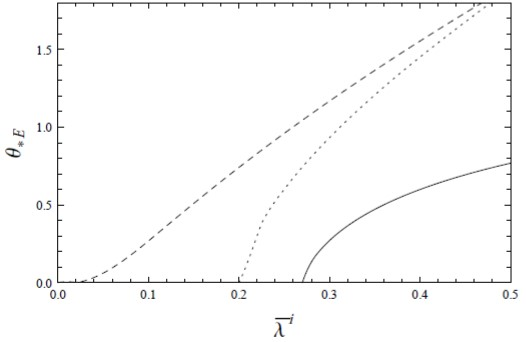
\includegraphics[width=0.4\textwidth]{Figura 2.jpg}
    \caption{The Einstein radius, $\theta_{*E}$, as function of $\bar{\lambda}^{i}$, for SFDM (solid line), NFW (dashed line), and Burkert (dotted line) halo models. Einstein rings of similar magnitude require $\bar{\lambda}^{NFW} < \bar{\lambda}^{Burkert} < \bar{\lambda}^{SFDM}$.}
    \label{Fig. 2}
\end{figure}

$\bar{\lambda}$ in order to produce Einstein rings of similar magnitude to those obtained for the other profiles, but this is in part due to projection effects that have not been considered in this paper [13, 18].

\section[III]{\centering \small {LENSING VS DYNAMICS}}
Taking into account that in SFDM models there is a critical value for the parameter $ \bar{\lambda},~\bar{\lambda}_{cr}\simeq0.27$, and considering the definition in Eq. (\ref{eq:5b}), we can write the condition to produce strong lensing in the form

\begin{equation}
\tag{6}\label{eq:6}
\rho_{c}r_{max}[M_{\odot}pc^{-2}]\gtrsim473.68hf_{dist},
\end{equation}

with $f_{dist}\equiv d_{OS}/d_{OL}d_{LS}$ a distance factor.
In order to evaluate the right-hand-side (r.h.s.) of Eq. (\ref{eq:6}), we consider two surveys of multiply-imaged systems,
the CASTLES \cite{19} and the SLACS 20]. From them we select only those elements for which the redshifts of the source and the lens have been determined (which amounts to approximately 60 elements in each survey), and calculate the corresponding distance factor $f_{dist}$ for every element in the reduced sample. In CASTLES (SLACS) the distance factors are in the interval $4 \lesssim f_{dist} \lesssim 27, (6 \lesssim f_{dist} \lesssim 25)$, with a mean value of $f_{dist} \simeq 7, (f_{dist} \simeq 11)$, and then the r.h.s. of Eq. (\ref{eq:6}) takes on values in the range 1400 - 9000, (2000 - 8500). Some representative elements from SLACS are shown in Table \ref{tab:1} (galaxy lensing). In terms of the mean values, the inequality in Eq. (\ref{eq:6}) translates into
\begin{subequations}
    \begin{equation}
    \tag{7a} \label{eq:7a}
             \rho_{c}r_{max}[M_{\odot}\text{pc}^{-2}]\gtrsim2000,~\text{(CASTLES)}
    \vspace{-1em}     
    \end{equation}
    \begin{equation}
    \tag{7b}\label{eq:7b}
             \rho_{c}r_{max}[M_{\odot}\text{pc}^{-2}]\gtrsim4000,~\text{(SLACS)}
    \end{equation}
\end{subequations}

These numbers are an order of magnitude greater than those obtained from dwarf galaxies dynamics, $\rho_{c}r_{max}[M_{\odot}\text{pc}^{-2}]\simeq100$  when interpreted using the same density profile \cite{7}; see again Table \ref{tab:1}. This is the main result of the paper. Remember that the value of $r_{max}$ is related to the fundamental parameters of the model, which are the mass of the scalar particle and the self-interaction term, and it remains constant throughout the formation
of cosmic structure. 
We must recall that inequalities in Eq. (7) do not take into account the presence of baryons in galaxies. Gravity does not distinguish between luminous and dark matter; then the contribution of the former to the lens could be significant in some cases. For instance, for those systems in SLACS the stellar mass fraction within the Einstein radius is 0.4, on average, with a scatter of 0.1 \cite{21}. We have corroborated that our estimates in Eq. (7) are not sensitive to the inclusion of a baryonic component. To see that we add the contribution of a de Vacouler surface brightness profile \cite{22} to the lens equation,

\begin{equation}
    \tag{8a}\label{eq:8a}
    \beta_{*}(\theta_{*})=\theta_{*}-\bar{\lambda}\frac{m(\theta_{*})}{\theta_{*}}-\bar{\lambda}_{lum}\frac{f(\theta_{*}/r_{e*})}{\theta_{*}}
\end{equation}

Here $\bar{\lambda}_{lum}$ is a paramater analogous to that given in Eq (5b),
\begin{equation}
    \tag{8b}\label{eq:8b}
    \bar{\lambda}_{lum}\equiv\frac{(M/L)L}{2\pi\Sigma_{cr}}
\end{equation}
and f(x) a dimensionless projected stellar mass,
\begin{equation}
\begin{split}
\tag{8c}\label{8c}
    f(x)=\frac{1}{2520}[e^{q}(q^{7}-7q^{6}+42q^{5}-210q^{4}+840q^{3}\\
    -2520q^{2}+5040q-5040)],
\end{split}
\end{equation}

with $q\equiv -7.76x^{-1/4}$. The mass-to-light ratio, $M/L$ (from a Chabrier initial mass function), and the effective radius, $r_{e}$, for each system in SLACS are reported in Ref. \cite{21}. With the use of Eq. (8) strong lensing is always
possible. Consequently, we must impose a different condition to constrain the product $\rho_{c}r_{max}$ in each galaxy, such as demand the formation of Einstein rings of certain radius.
To proceed we use a small subsample of SLACS that includes configurations with the minimum, maximum, and mean Einstein radius, and stellar surface mass density,
respectively. This is because the new lens equation is a function of the ratio $r_{e*} = r_{e}/ r_{max}$; then, to compute the magnitudes of the Einstein radii, we shall fix the value of $r_{max}$ a priori.
Using the new lens equation we find the value of $\bar{\lambda}$ that produces the appropriate Einstein radius for each of the elements in the subsample. This is done using two different values of $r_{max}$: 5 and 10 Kpc. The resultant products $\rho_{c}r_{max}$ are compatible (in order of magnitude) with the inequalities obtained from Eq. (\ref{eq:6}). Only for those systems in the subsample with a high stellar surface mass density the value of $\rho_{c}r_{max}$ can decrease substantially, but it is important to have in mind that all the possible uncertainties associated to the distribution of the luminous matter, like the choice of the stellar initial mass function, will be more relevant in such cases. In general, these estimations are sensitive to the details of the particular configuration, and a more exhaustive analysis, considering the complete sample, will be presented elsewhere.

\begin{table*}[t]
  \centering
        \begin{tabular}{ |p{2cm}|p{3cm}|p{2cm}|p{1cm}|p{3cm}|}
         \hline
         \multicolumn{2}{|c|}{\textbf{DYNAMICS OF GALAXIE}} 
         &\multicolumn{3}{|c|}{\textbf{GALAXY LENSING}} \\
         \hline
         Galaxy & $\rho_cr_{max}$[$M_{odot}\text{pc}^{-2}$] & Galaxy & $f_{dist}$ & $\rho_cr_{max}$[$M_{odot}\text{pc}^{-2}$] \\ 
         \hline
         HO II   & 36.19 & J0008-0004 & 6.61 & 2029.68\\
         \hline
         DD0 154 & 66.47 & J1250+0523 & 8.46 & 2832.41\\
          \hline
         DDO 53 & 67.53 & J2341+0000 & 9.12 & 3053.38\\
          \hline
         IC2574 & 81.89 & J1538+5817 & 11.74 & 39.30.44\\
          \hline
         NGC2366 & 85.45 & J0216-0813 & 13.03 & 4362.44\\
          \hline
         Ursa Minor & 104.72 & J1106+5228 & 15.74 & 5269.75\\
          \hline
         Ho I &120.23 & J2321-0939 & 16.23 & 5433.80\\
         \hline
         DD0 39 & 145.94 & J1420+6019 & 19.72 & 6602.26\\
         \hline
         M81dwB & 265.87 & J0044+0113 & 25.26 & 8547.05\\
         \hline
         \end{tabular}
                  \vspace{1em}
         \caption{Estimates of the product $\rho_{c}r_{max}$ for different galaxies. \textit{Left}. As reported in Refs. \cite{7}, using galactic dynamics. \textit{Right}. Derived from equation (\ref{eq:6}) in this paper; recall that these values represent a lower limit (here we show only a representative subsample of the SLACS survey). Note the difference of an order of magnitude between the values of $\rho_{c}r_{max}$ for dwarf galaxies in the local universe, and the lower limit of this same quantity for galaxies producing strong lensing at $z\sim 0.5$.}
        \label{tab:1}
    \end{table*}

\section[IV]{\centering \small {DISCUSSION AND FINAL REMARKS}}
We have shown that a discrepancy between lensing and
dynamical studies appears if we consider that the SFDM
mass density profile in Eq. (\ref{eq:1}) describes the inner regions
of galactic halos at different redshifts, up to radii of order
5-10Kpc. More specifically, we have found that lens
galaxies at $z\sim 0.5$, if correctly described by a SFDM halo
profile, should be denser than dwarf spheroidals in the
local universe, in order to satisfy the conditions necessary
to produce strong lensing.
In principle nothing guarantees that halos of different
kind of galaxies share the same physical properties.
Our studies took into account galaxies that are intrinsically
different in terms of their total mass and baryon
concentration. While dwarf galaxies show low stellar surface
brightness, stellar component in massive, early type
galaxies is typically compact and dense.
In the standard cosmological model the evolution of
DM halos may trigger differences in concentrations for
halos with different masses due to differences in the assembling
epoch; smaller halos collapsed in an earlier and
denser universe, therefore they are expected to be more
concentrated. However, it is also well known that the
presence of baryons during the assembly of galaxies can
alter the density profile of the host halos and modify
this tendency, making them shallower (supernova feedback
\cite{22}), or even cuspier (adiabatic contraction \cite{24}).
Therefore, the stellar distribution may reveal different
dynamical evolution for low and high mass halos triggered
by galaxy formation.
For SFDM, the dynamical interaction between baryons
and the scalar field may also modify the internal halo
structure predicted by the model, Eq. (\ref{eq:1}), clarifying the
discrepancy. For instance, if the concentration of stellar
distribution were correlated with that of the halo,
like in the adiabatic contraction model when applied to
standard DM halos, this may explain our findings. But
at this time it is unknown how compressible SFDM halos
are, and if such effect will be enough to explain our
results, because there are no predictions on its magnitude.
If the modification triggered by baryons were insufficient, then it might be suggesting an intrinsic evolution
of SFDM halos across cosmic time. For example, if big
galaxies emerge as the result of the collision of smaller
ones, then the central densities of the resultant galaxies
would be naturally higher; after all, $r_{max}$ is a constant
in the model, and one would expect that total mass is
preserved in galaxy-galaxy mergers. At this point we do
not know which of these two mechanisms, the intrinsic to
the model, or that due to the evolution of SFDM halos
in the presence of baryons, is the dominant one. In that
sense, a theoretical description of these processes may be
very useful and welcome.
A full picture requires a distribution of values for the
central density generated from the evolution of the spectrum
of primordial density perturbations after inflation.
Such a result is not available now, but it is possible to
start tracing this distribution with galaxy observations.
We present, for the first time, observational constraints
on the dynamical evolution of SFDM halos in the presence
of baryons, that must be considered for future semianalytical/
numerical studies of galaxy formation.\\ 

\renewcommand{\abstractname}{\center\small {ACKNOWLEDGMENTS}}
\begin{abstract}
\\\\We are grateful to Juan Barranco for useful comments.
This work was partially supported by PROMEP, DAIPUG,
CAIP-UG, PIFI, I0101/131/07 C-234/07 of the Instituto
Avanzado de Cosmología (IAC) collaboration,
DGAPA-UNAM grant No. IN115311, and CONACyT
México under grants 167335, 182445. AXGM is very
grateful to the members of the Departamento de Física
at Universidad de Guanajuato for their hospitality.
\end{abstract}

\newpage
\bibliographystyle{abbrv}
\bibliography{references}


\end{document}
